\documentclass[tikz]{standalone}
\usepackage{palatino}
\begin{document}
	\begin{tikzpicture}[font=\Large]
		\node[anchor=south west,inner sep=0] (image) at (0,0) {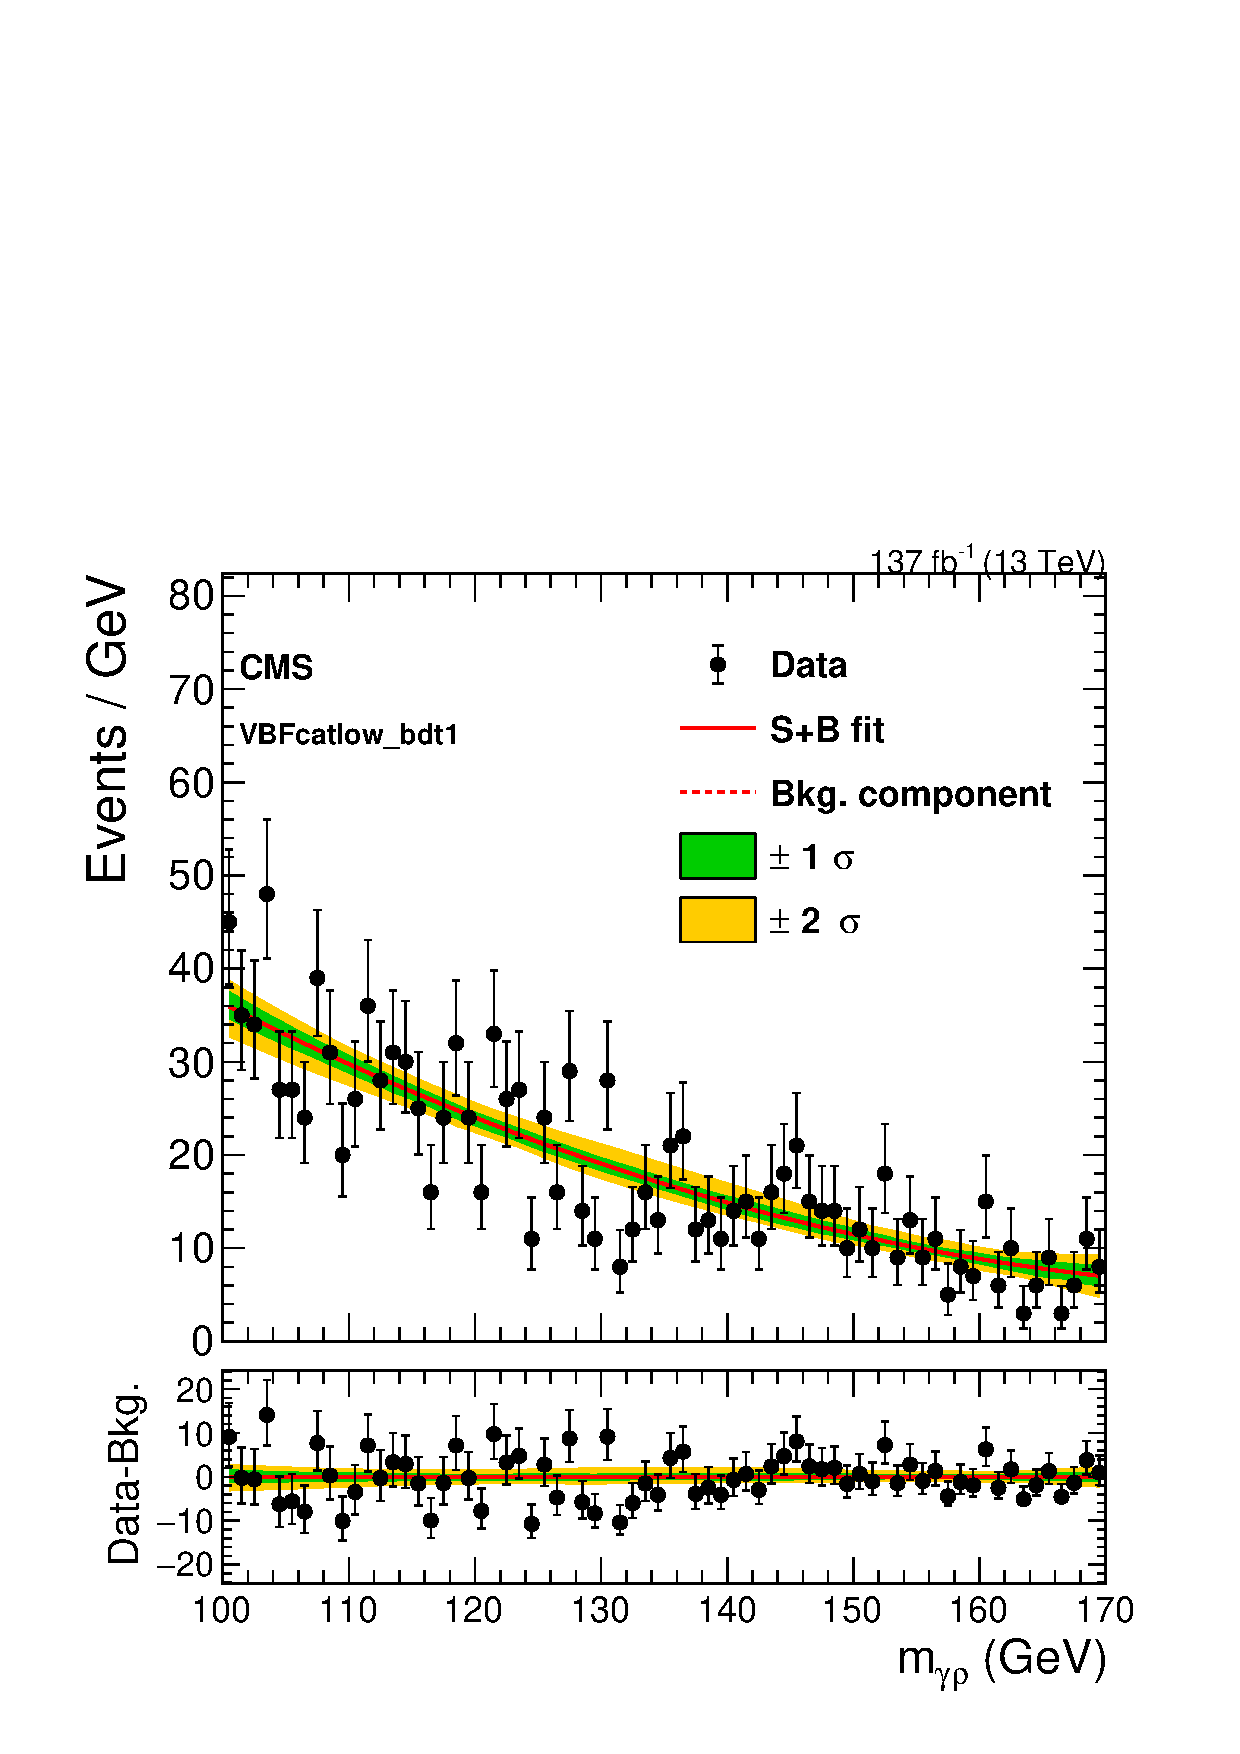
\includegraphics[width=\textwidth]{../23-004-v08-figs/mass_postfit_VBFcatlow_bdt1_Rho.pdf}};
		\begin{scope}[x={(image.south east)},y={(image.north west)}]
			\draw[blue,ultra thick] (-0.004,-0.008) rectangle (0.997,0.997);
			\draw[blue,ultra thick] (-0.004,-0.008) rectangle (0.16,0.058);
			\draw (0,0) node[anchor=south west] {\textcolor{blue}{\textbf{TWiki}}};
		\end{scope}
	\end{tikzpicture}
\end{document}